Das Ziel des Command-Pattern ist, den Requests und Receiver von dem Invoker auszulagern um diese flexibel austauschbar zu gestalten. Hierzu wird eine zusätzliche Schicht eingeführt, nämlich das Command-Objekt. In einem  Szenario ohne dem Command-Pattern, würde der Invoker den Receiver als Objekt besitzen um darauf dessen Methoden aufzurufen. Dadurch ergibt sich allerdings, das der Receiver an den Invoker gebunden ist. Um das dieses Problem zu lösen, führt man auf der Seite des Invokers eine Schnittstelle, \texttt{Command} ein, die eine Methode \texttt{execute()} besitzt. Auf der andere Seite erstellt man ein konkretes Objekt, das von dieser Schnittstelle erbt und gleichzeitig den Receiver kennt, um dort diesen zu verwenden. Der Invoker muss also nur ein passendes Command-Objekt erhalten und  dessen Methode \texttt{execute()} aufrufen. Die konkrete Durchführung dieser Methode wird  dann in dem konkreten Command-Ojbekt behandelt. Abbildung \ref{commanddiagramm} zeigt ein UML-Diagramm für das Command-Pattern.


\begin{figure}[htbp]
\centering
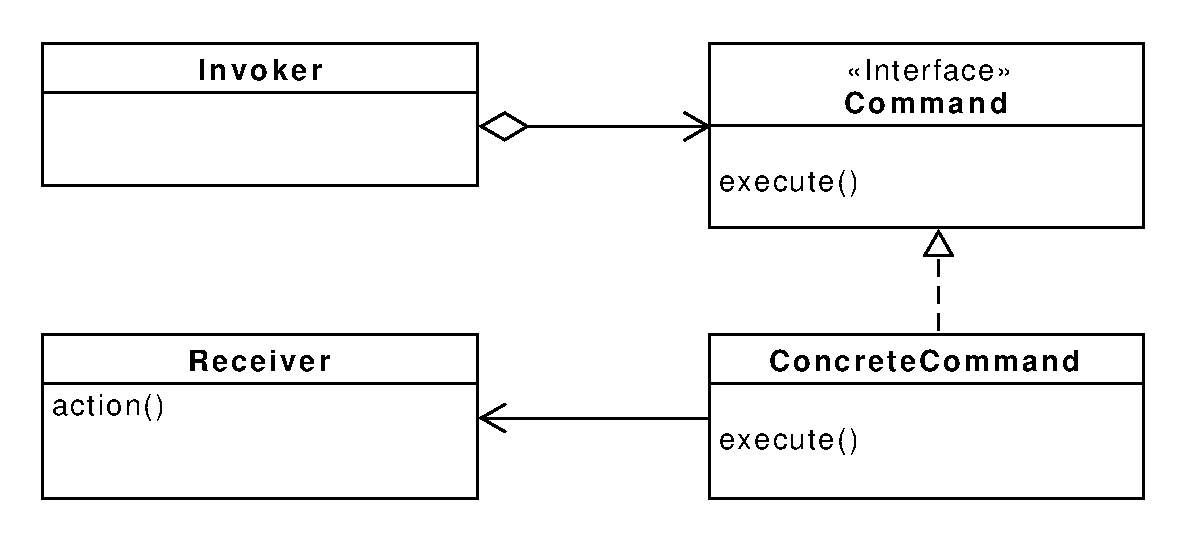
\includegraphics[width=0.7\textwidth]{./paper/command/command}
\caption{Command-Pattern als UML-Diagramm.}
\label{commanddiagramm}
\end{figure} 